%pdflatex main.tex
\documentclass[12pt]{article}
\usepackage{natbib}
\usepackage[francais]{babel}
\usepackage{natbib}
\usepackage{url}
\usepackage[utf8x]{inputenc}
\usepackage{amsmath}
\usepackage{graphicx}
\usepackage{float}
\graphicspath{{images/}}
\usepackage{amsthm}
\usepackage{parskip}
\usepackage{fancyhdr}
\usepackage{xfrac}
\usepackage{esvect}
\usepackage{vmargin}
\usepackage{gensymb}
\setmarginsrb{3 cm}{2.5 cm}{3 cm}{2.5 cm}{1 cm}{1.5 cm}{1 cm}{1.5 cm}

\title{Points de Lagrange}								% Title
\author{Groupe 5}								% Author
\date{\today}											% Date

\makeatletter
\let\thetitle\@title
\let\theauthor\@author
\let\thedate\@date
\makeatother

\pagestyle{fancy}
\fancyhf{}
\rhead{\theauthor}
\lhead{\thetitle}
\cfoot{\thepage}
\newtheorem*{rappel}{Rappel}
\newtheorem*{nota}{N.B}
\newtheorem*{req}{Remarque}
\begin{document}

%%%%%%%%%%%%%%%%%%%%%%%%%%%%%%%%%%%%%%%%%%%%%%%%%%%%%%%%%%%%%%%%%%%%%%%%%%%%%%%%%%%%%%%%%

\begin{titlepage}
	\centering
    \vspace*{0.5 cm}
    
\includegraphics[scale = 0.75 ]{logo1.png}\\[1.0 cm]	% University Logo
    \textsc{\LARGE EISTI}\\[2.0 cm]			% University Name
    \rule{\linewidth}{0.2 mm} \\[0.5 cm]
    { \huge \bfseries \thetitle}\\
    \rule{\linewidth}{0.2 mm} \\[1.5 cm]
	\textsc{\Large Atelier}\\[0.5 cm]	% Course Code
	\textsc{\large CPI1 C2 - Groupe 5}\\[0.5 cm]		% Course Name
	
	\begin{minipage}{0.4\textwidth}
	\centering
		\begin{center} \large
		Maxime LUNDQUIST \\
		Mandry MBUNDU \\
		David RIGAUX \\
		Mehdi DALAA \\
			\end{center}
			\end{minipage}~
			\begin{minipage}{0.4\textwidth}
	\end{minipage}\\[0.8 cm]
	{\large \thedate}\\[1 cm]
	\vfill
	
\end{titlepage}

%%%%%%%%%%%%%%%%%%%%%%%%%%%%%%%%%%%%%%%%%%%%%%%%%%%%%%%%%%%%%%%%%%%%%%%%%%%%%%%%%%%%%%%%%

\tableofcontents
\addtocontents{toc}{~\hfill\textbf{Page}\par}
\pagebreak

%%%%%%%%%%%%%%%%%%%%%%%%%%%%%%%%%%%%%%%%%%%%%%%%%%%%%%%%%%%%%%%%%%%%%%%%%%%%%%%%%%%%%%%%%

\section{Rappels}
\subsection{Gravité, loi d'attraction universelle}
La loi de l'attraction universelle, découverte par Isaac Newton, est la loi décrivant la gravitation comme une force responsable de la chute des corps et du mouvement des corps célestes, et de façon générale, de l'attraction entre des corps ayant une masse.
\\
Deux corps ponctuels de masses respectives M(A) et M(B) s'attirent avec des forces de mêmes valeurs (mais vectoriellement opposées), proportionnelles à chacune des masses, et inversement proportionnelles au carré de la distance qui les sépare. Cette force a pour direction la droite passant par les centres de gravité de ces deux corps. 
\\
$$F_{A/B} =F_{B/A} = G\frac{M_{A} * M_{B}}{d²}$$
\begin{align*}
\begin{tabular}{|p{10cm}}
$F_{A/B}$ et $F_{B/A}$ : force d'attraction en $N$ \\
$M_{A}$ et  $M_{B}$  : masse des deux corps en $kg$\\
$d$ : distance séparant les deux corps $m$ \\
$G$ : constante universelle de la gravitation : \\
$G = 6,67*10^{-11} m^{3}.kg^{-1}.s^{-2}$
\end{tabular}
\end{align*}
\\
Cette formule peut être retrouvée en partant de la troisième loi de Kepler : \\
\textbf{Troisième loi de Kepler} : Le carré de la période d'une planète autour du soleil est proportionnel au cube de la longueur du demi-grand axe de son orbite. 
\\
\begin{align*}
\frac{T^2}{a^3} &= k & \begin{tabular}{|p{10cm}}
$T$ : période de révolution de la planète en $s$ \\
$a$ : longueur du demi-grand axe de l'orbite en $m$\\
$k$ : coefficient de proportionnalité en $s^{2}.m^{3}$
\end{tabular}
\end{align*}
\\
\textbf{Ce rapport de proportionnalité est le même pour toutes les planètes du système solaire.}
\pagebreak
\subsection{Lois de la mécanique de Newton}
Les lois du mouvement de Newton sont les principes de base de sa grande théorie concernant le mouvement des corps, théorie que l'on nomme aujourd'hui Mécanique Newtonienne.
\subsubsection{Première loi de Newton, principe d'inertie}
Si un objet est au repos ou que son mouvement est rectiligne uniforme, alors la somme des forces extérieures qui s'exercent sur lui est nulle, et réciproquement :
\\
$$\sum \vv{F_{ext}} = \vv{0}$$
\subsubsection{Deuxième loi de Newton, principe fondamental de la dynamique de translation}
Le vecteur résultant de la somme des forces extérieures qui s'exercent sur le solide est colinéaire au vecteur accélération et ce quelque soit le mouvement de l'objet. Le coefficient de colinéarité correspond à la masse de l'objet, on a donc la relation suivante :
\\
\begin{align*}
\sum \vv{F}_{ext} &= m\vv{a} & \begin{tabular}{|p{10cm}}
$m$ : masse en $kg$ \\
$\vv{a}$ : vecteur accélération
\end{tabular}
\end{align*}
\subsubsection{Troisième loi de Newton, principe des actions réciproques}
Si un objet A exerce une force sur un objet B, alors cet objet B exerce une force sur A de même direction, de même intensité, mais de sens opposé :
\\
$$\vv{F}_{A/B} = -\vv{F}_{B/A}$$
\subsection{Force centrifuge/centripète: mouvement circulaire}
\begin{figure}[H]
\centering
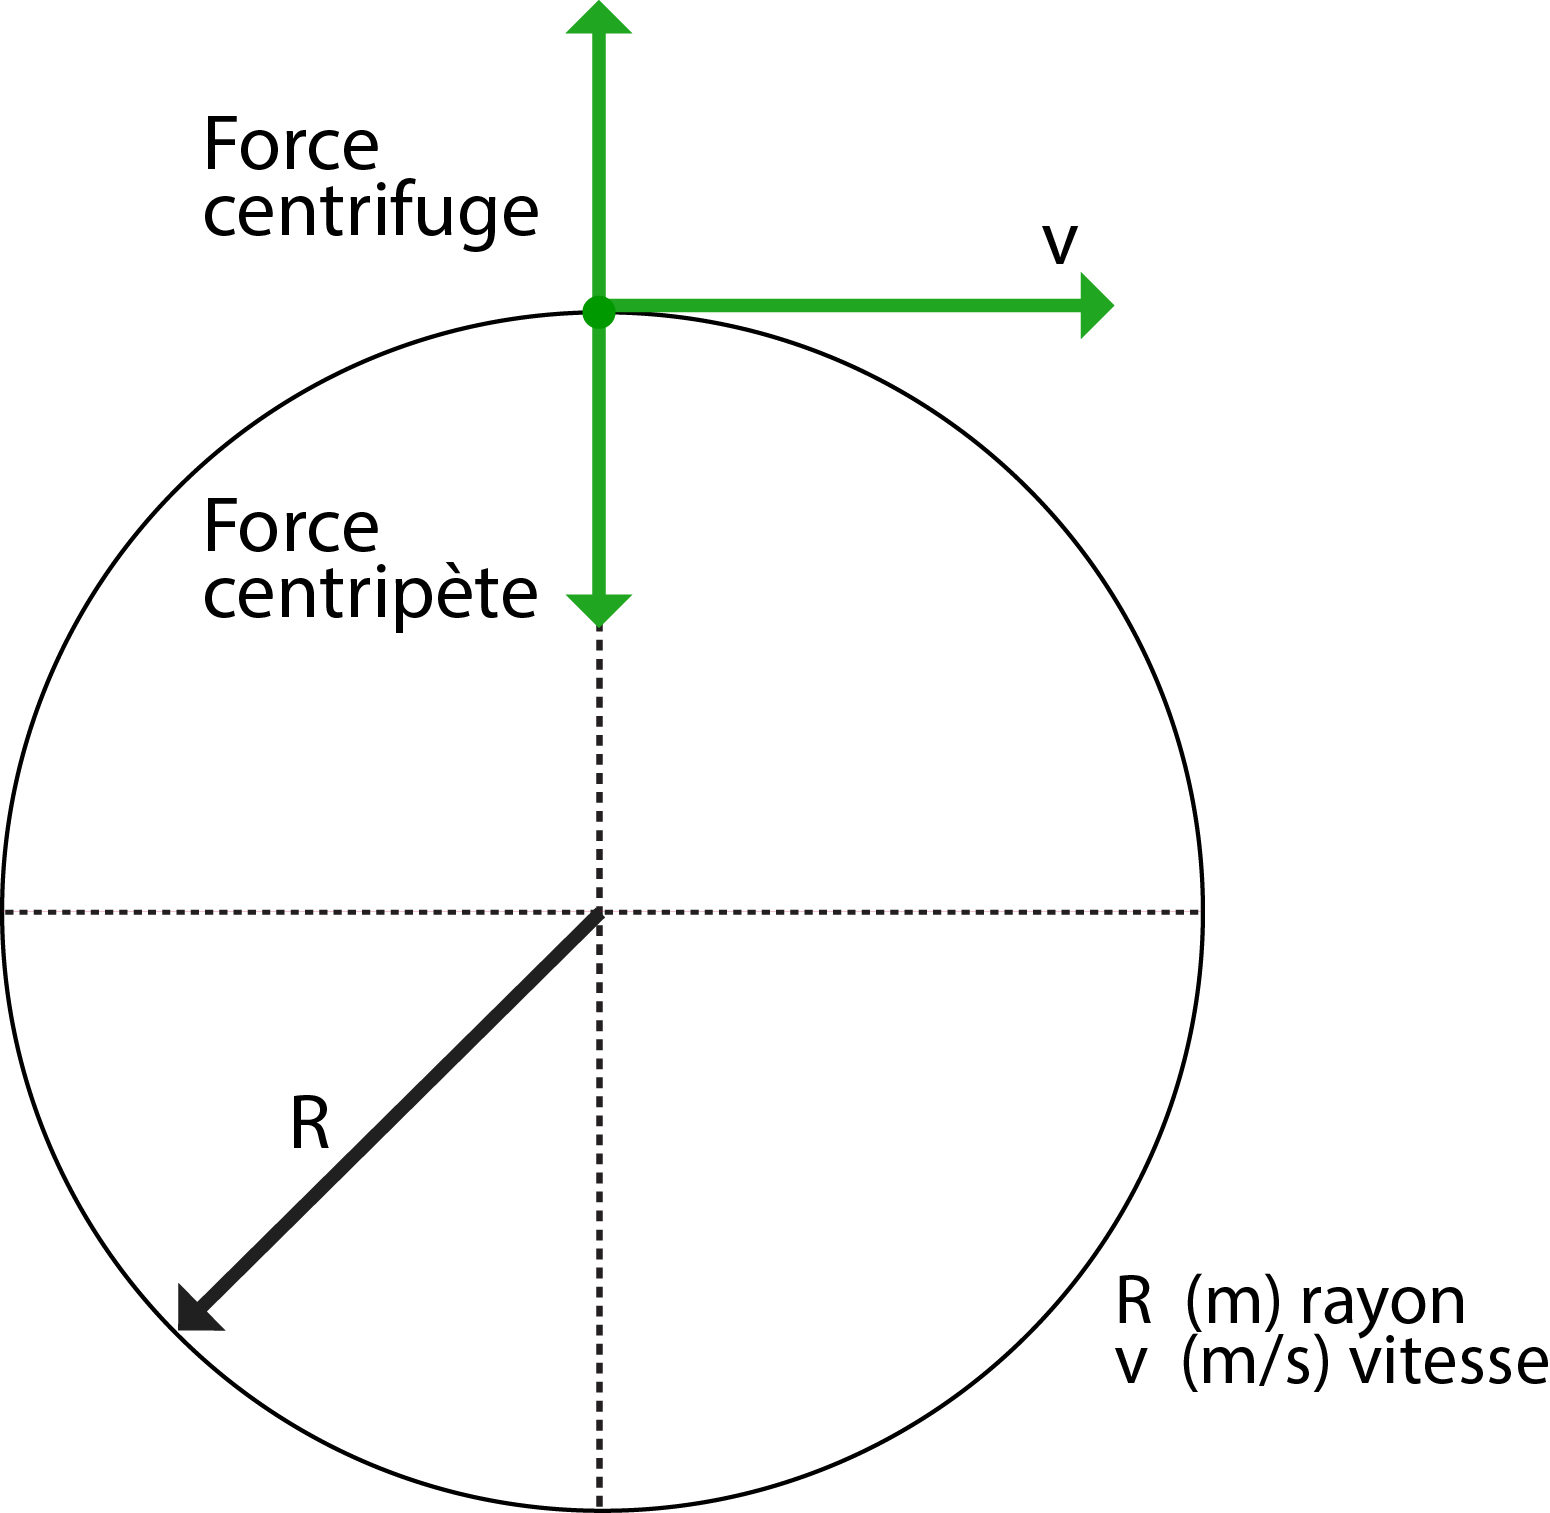
\includegraphics[width=0.5\textwidth]{centri.png}
\caption{Force centrifuge et centripète}
\end{figure}
Une force désigne toute cause capable de modifier la vitesse ou la trajectoire d’une masse et \textit{``centrifuge''} signifie qui éloigne du centre. \\
Le concept de force centrifuge est une application du principe général d’inertie au cas particulier du mouvement circulaire, mode de raisonnement imaginaire. Ainsi, une force qualifiée de centrifuge devrait pouvoir éloigner une masse quelconque d’un centre ou d’un axe de rotation selon une trajectoire radiale, c’est-à-dire dans la direction indiquée par le prolongement d’un rayon. \\
La force centrifuge est l'association de deux forces: l'inertie et la force centripète. C'est pourquoi on dit que la force centrifuge est une force fictive.
\\
\begin{align*}
F &= \frac{Mv}{R} & \begin{tabular}{|p{10cm}}
$F$ : force centrifuge en $N$ \\
$v$ : vitesse du corps en $m.s^{-1}$ \\
$R$ : rayon du cercle en $m$
\end{tabular}
\end{align*}
Centripète signifie \textit{``qui rapproche du centre''} donc une force est dite centripète quand son action consiste à rapprocher une masse d’un centre quelconque.
Il y a seulement deux forces de nature centripète: \\
\begin{itemize}
\item La force électromagnétique : elle permet à un atome lourd de capturer un ou plusieurs atomes plus légers pour constituer une molécule;
\item La force de gravitation : c'est une attraction de même nature qui maintient la Terre en orbite autour du Soleil. La masse du Soleil délivre une force qui dévie la trajectoire de la Terre. Si cette force n’existait pas, la Terre quitterait le système solaire. Et si la vitesse de la Terre était nulle, celle-ci prendrait immédiatement la direction du Soleil.
\end{itemize}
\begin{align*}
F &= \frac{Mv^2}{R} & \begin{tabular}{|p{10cm}}
$F$ : force centripète en $N$ \\
$v$ : vitesse du corps en $m.s^{-1}$ \\
$R$ : rayon du cercle en $m$
\end{tabular}
\end{align*}
\section{Points de Lagrange}
Un point de Lagrange est une position de l'espace où les champs de gravité de deux corps en orbite l'un autour de l'autre, de masses conséquentes, fournissent exactement la force centripète requise pour que ces points de l'espace accompagnent simultanément l'orbite des deux corps. \\
Dans le cas où les deux corps sont en orbite circulaire, ces points représentent les endroits où un troisième corps de masse négligeable resterait immobile par rapport aux deux autres, au sens où il accompagnerait à la même vitesse angulaire leur rotation autour de leur centre de gravité commun, sans que sa position par rapport à eux n'évolue.

\begin{figure}[H]
\centering
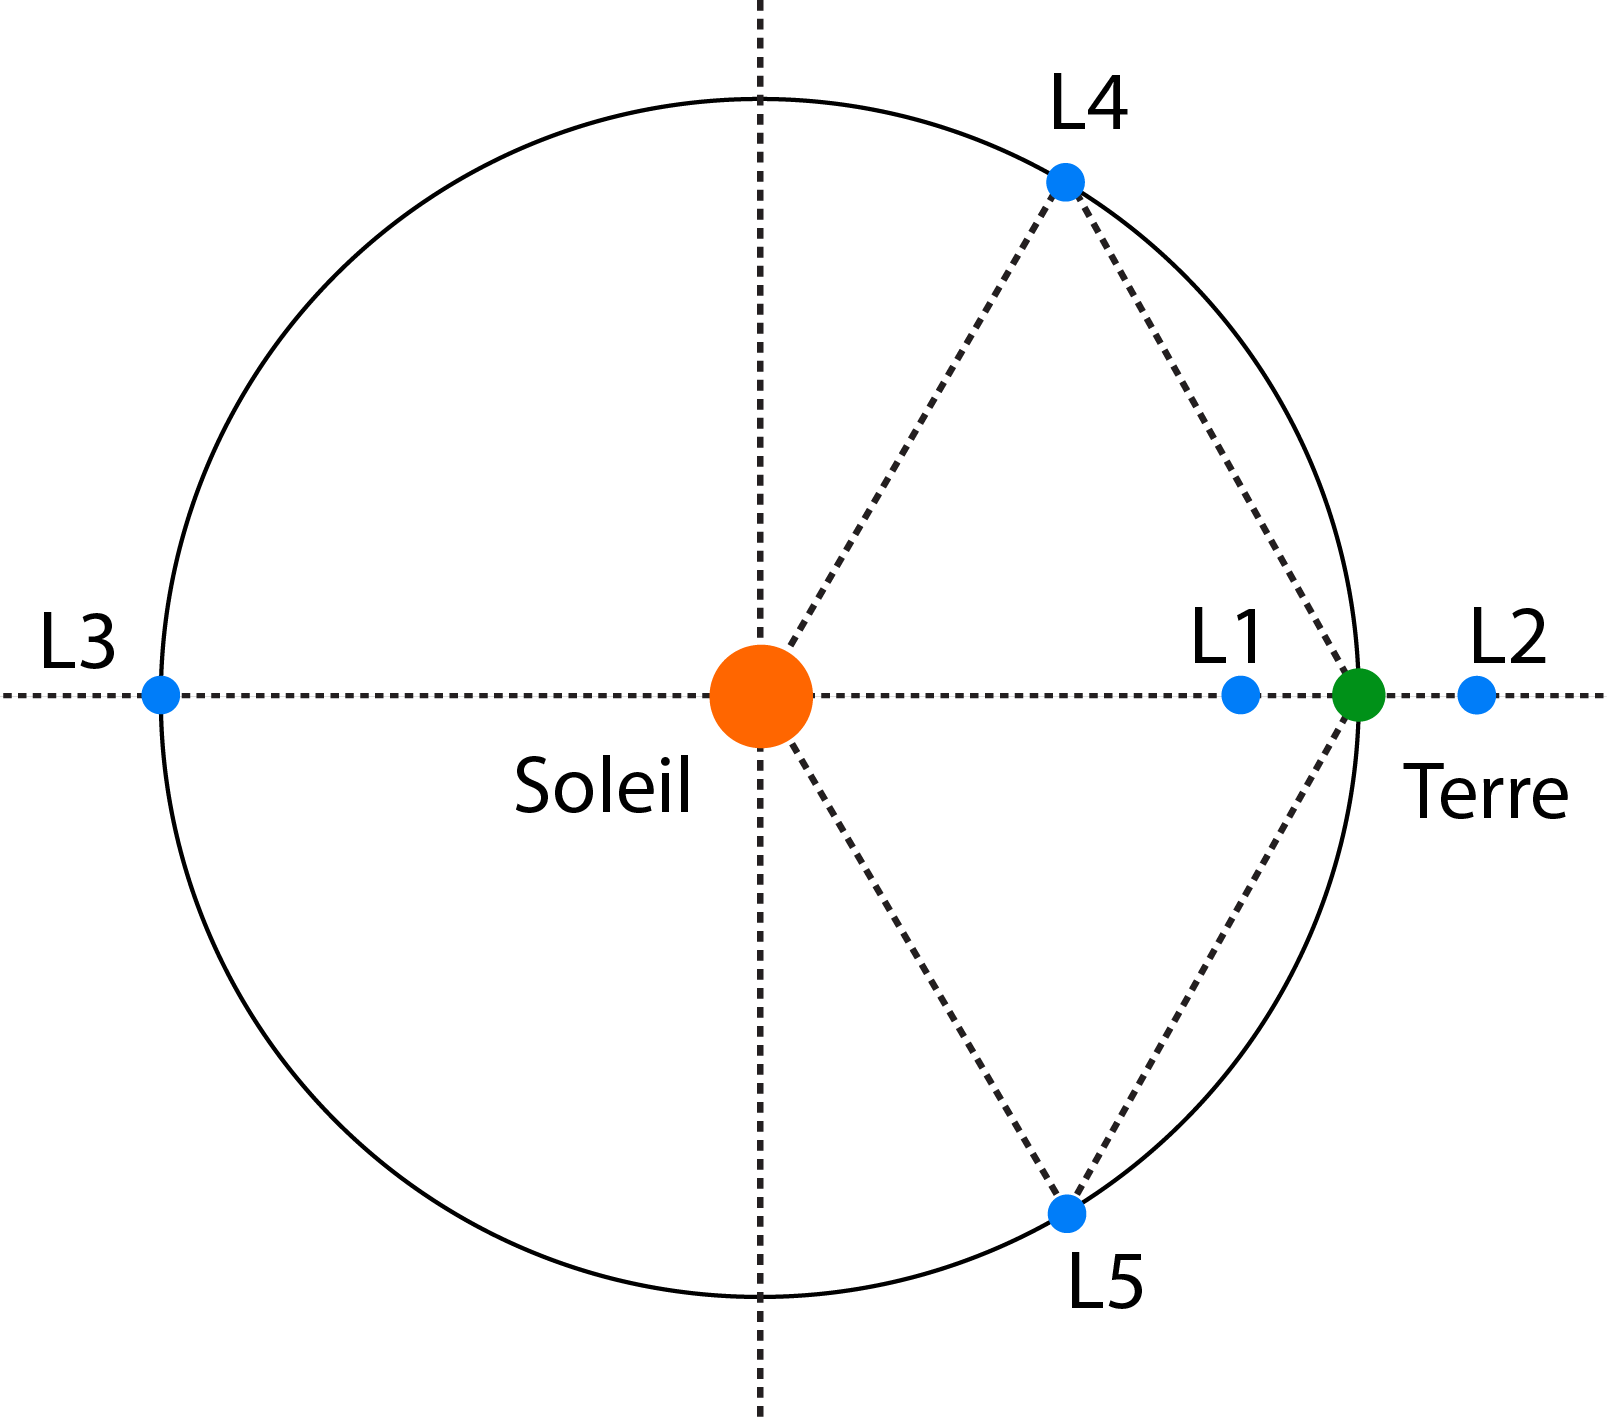
\includegraphics[width=0.64\textwidth]{lagrange.png}
\caption{Points de Lagrange}
\end{figure}

\section{Calculs des points de Lagrange} 
\subsection{L1}
\begin{figure}[H]
\centering
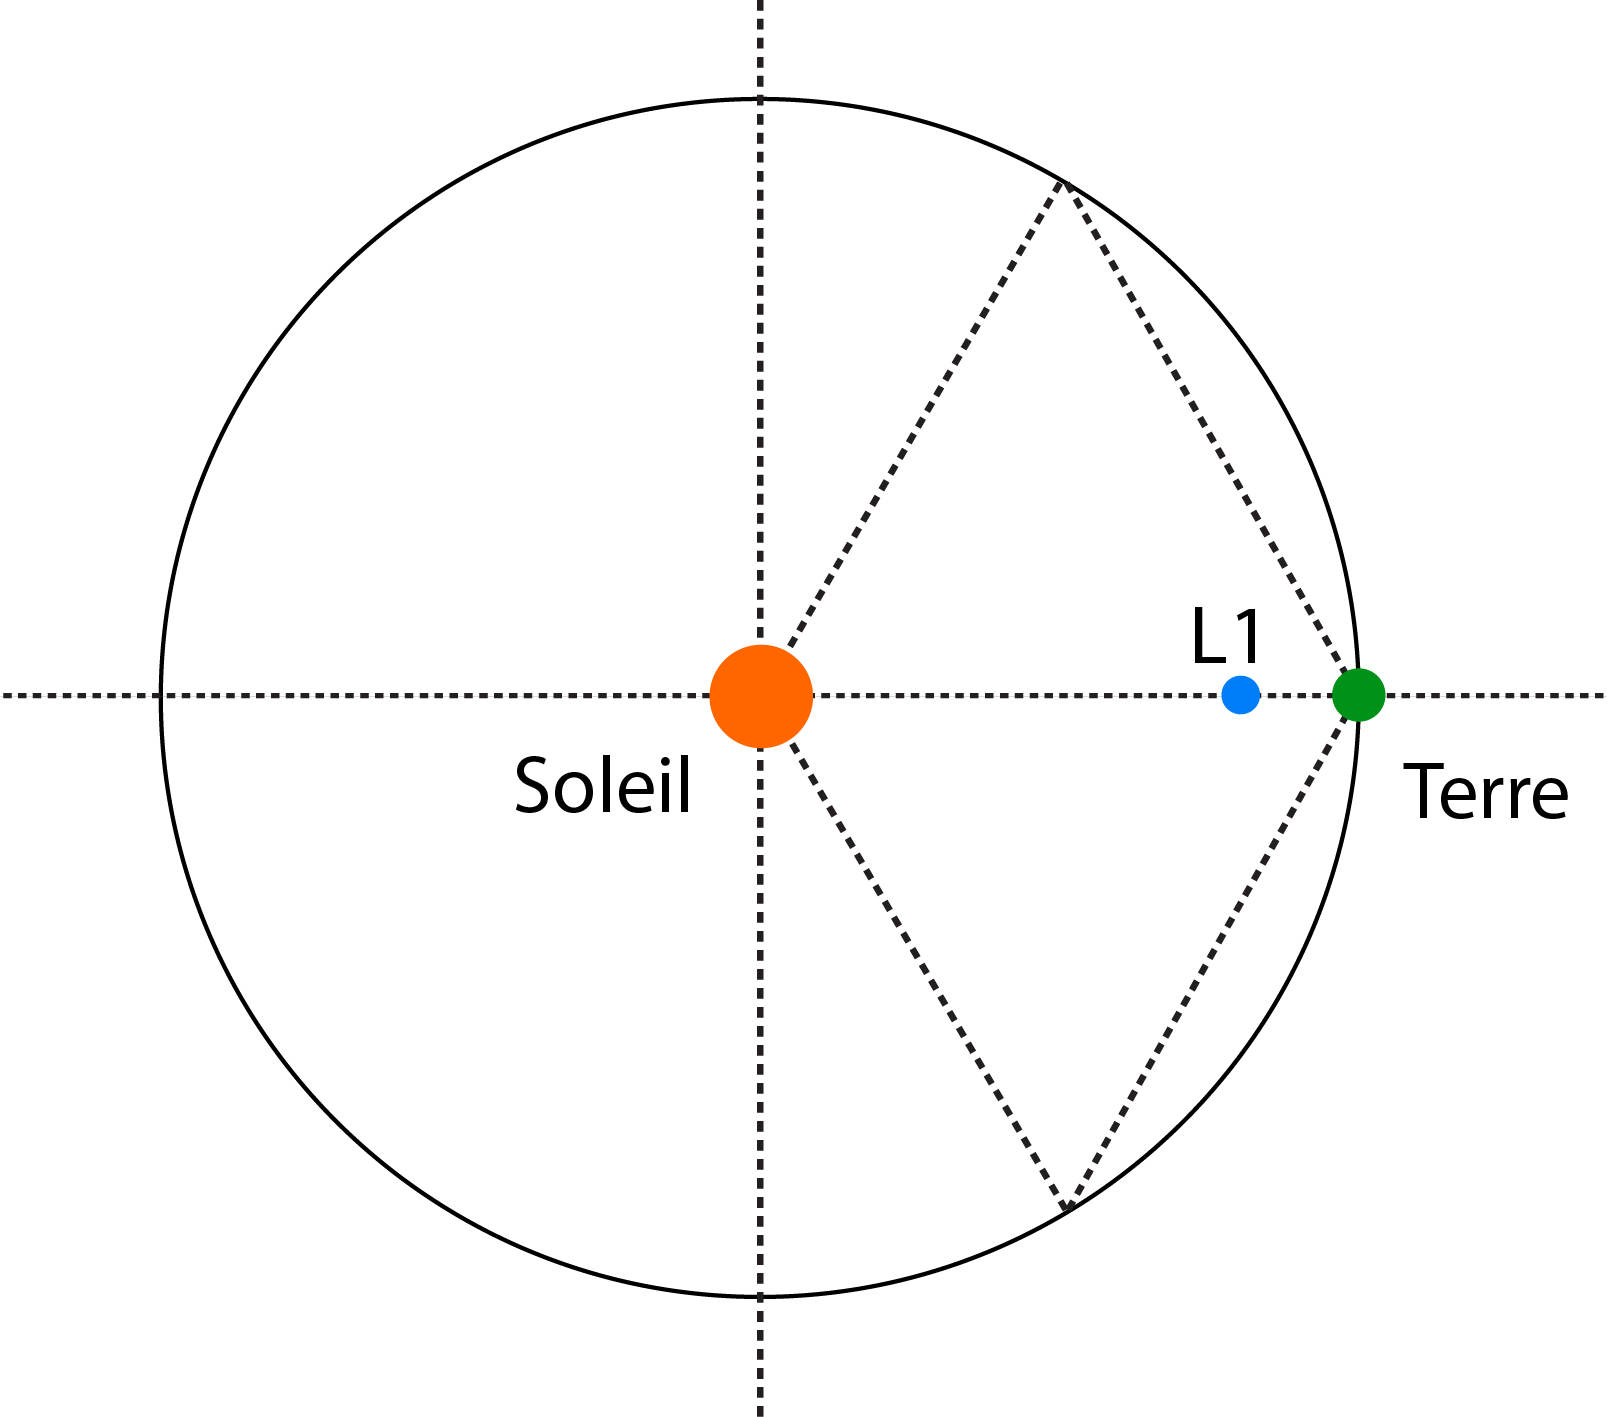
\includegraphics[width=0.6\textwidth]{L1.png}
\caption{Point L1}
\end{figure}
La force d'attraction du Soleil notée $F_{s}$ représente la force grâce à laquelle le Soleil attire un satellite en fonction de sa masse, celle du Soleil et la distance séparant les deux corps :
\begin{align*}
\vv{F}_{S} &= \frac{GM_{0}m}{(R-r)^{2}} & \begin{tabular}{|p{10cm}}
$m$ : masse du satellite en $kg$ \\
$M_{0}$ : masse du soleil en $kg$ \\
$R$ : distance Terre-Soleil en $m$ \\
$r$ : distance Terre-Satellite en $m$
\end{tabular}
\end{align*}

La force d'attraction terrestre notée $F_{t}$ représente la force grâce à laquelle la Terre attire un satellite en fonction de la masse du satellite, celle de la Terre et la distance les séparant : 
\begin{align*}
\vv{F}_{T} &= \frac{GMm}{r^{2}} & \begin{tabular}{|p{10cm}}
$m$ : masse du satellite en $kg$ \\
$M$ : masse de la Terre en $kg$
\end{tabular}
\end{align*}

La force centripète notée $F_{c}$ désigne la force permettant de maintenir la Terre dans une trajectoire elliptique par rapport au Soleil : 
\begin{align*}
\vv{F}_{C} &= \frac{mv^{2}}{(R-r)} & \begin{tabular}{|p{10cm}}
$m$ : masse du corps en $kg$ \\
$v$ : vitesse du corps en $m.s^{-1}$ \\
$M$ : masse de la Terre en $kg$ \\
$R$ : distance Terre-Soleil en $m$ \\
$r$ : distance Terre-Satellite en $m$
\end{tabular}
\end{align*}

La période de révolution d'un corps céleste est la période durant laquelle ce corps fait le tour complet d'un autre corps autour duquel il gravite. \par
Période de révolution de la Terre autour du Soleil :    $v*T = 2\pi(R-r)$ \\
\begin{align*}
&\Rightarrow v = \frac{2\pi(R-r)}{T}  \hspace{0.5cm} or \hspace{0.5cm} \vv{F}_{C} = \frac{mv^{2}}{(R-r)} \\
&Or\hspace{0.3cm}v*T = 2\pi(R-r) \Rightarrow \vv{F}_{C} = \frac{m\left(4\pi^{2}(R-r)^{2}\right)}{T^2(R-r)}\\
&\vv{F}_{S} = \vv{F}_{C} + \vv{F}_{T}  \Rightarrow \frac{GM_{0}m}{(R-r)^{2}} = \frac{m(4\pi^{2}(R-r)^{2})}{T^2(R-r)} + \frac{GMm}{r^{2}}\\
&\frac{m(4\pi^{2}(R-r)^{2})}{T^2(R-r)} =  \frac{GM_{0}m}{(R-r)^{2}} - \frac{GMm}{r^{2}} \\
& \boxed{\frac{4\pi^{2}}{T^2} = \frac{GM_0}{(R-r)^3} - \frac{GM}{r^2(R-r)}} \tag{1}
\end{align*} \\
Nous considérons la Terre dans une situation d'équilibre entre la force d'attraction que le Soleil exerce sur elle et la force centrifuge engendrée par le mouvement circulaire de sa révolution solaire : \par
\begin{align*}
&donc\hspace{0.3cm}\vv{F}_{S/T} = \frac{Mv^2}{R} \\
&\Leftrightarrow \frac{GM_{0}M}{R^2} = \frac{M(2\pi R)^2}{RT^2}\hspace{0.5cm}car\hspace{0.3cm}v = \frac{2\pi R}{T} \Leftrightarrow v^2 = \frac{(2\pi R)^2}{T^2} \\
&\Leftrightarrow \frac{GM_{0}M}{R^2} = \frac{M4\pi^2 R^2}{RT^2} \\
&\Rightarrow \boxed{\frac{GM_{0}M}{R^2} = \frac{MV^2}{R} = \frac{M4\pi ^2 R^2}{RT^2}} \tag{2}
\end{align*} \\
On a alors :
\begin{gather*}
\frac{GM_{0}M}{(R-r)^{2}} = \frac{M4\pi ^2 R^2}{RT^2} \Rightarrow \frac{GM_{0}}{R^2} = \frac{4 \pi ^2 R}{T^2} \Rightarrow \frac{GM_{0}}{R^3} = \frac{4 \pi ^2}{T^2}
\end{gather*}
D'où :
\begin{equation*}
\boxed{\frac{GM_{0}}{(R-r)^3} - \frac{GM}{r^2(R-r)} = \frac{GM_0}{R^3}} \tag{3}
\end{equation*} \\

\[ \text{Posons} : 
\begin{cases}
y = \frac{M}{M_0}  & \quad \text{ qui est une très petite valeur}\\
z = \frac{r}{R}  & \quad \text{ qui est une petite valeur}\\
\end{cases}
\]
(3) devient alors :
\begin{align*}
& \frac{G}{(R-r)^3} - \frac{G}{r^2 (R-r)} * \frac{M}{M_0} = \frac{G}{R^3}\\
\Rightarrow \, &\frac{1}{(R-r)^3} - \frac{1}{r^2(R-r)} * y = \frac{1}{R^3} \\
\Rightarrow \,&\frac{1}{R^3(1-\frac{r}{R})} - \frac{1}{r^2R(1-\frac{r}{R})}*y = \frac{1}{R^3}  \\
\Rightarrow \,&\frac{1}{(1-\frac{r}{R})^3} - \frac{R^2}{r^2} * \frac{1}{(1-\frac{r}{R})}*y= 1 \\
\Rightarrow \,&\frac{1}{(1-z)^3}-\frac{y}{z^{2}(1-z)} = 1 \\ \\
&z \text{ est une très petite valeur, }(1-z) \rightarrow 1 \text{ (car } z \sim 0 \text{)}  \\
\Rightarrow \,&\frac{1}{(1-z)^3} -  \frac{y}{z^2} = 1
\end{align*} \\

En effectuant le développement limité de $\frac{1}{(1-z)^3}$ à l'ordre 1, on a : 
\begin{align*}
&1+3z-\frac{y}{z^2} = 1 \\
\Rightarrow \, &z^2 + 3z^3 -y =z^2 \\
\Rightarrow \, &\boxed{3z^3 = y} \quad \text{Donc (3)} \Leftrightarrow 3z^3 = y 
\end{align*} \\
Nous nous intéressons à la distance $r$ séparant $L1$ et la Terre. \\
À partir de $(3)$, nous avons : \\
\begin{align*}
3z^3 = y \Rightarrow \, &3\frac{r^3}{R^3} = \frac{M}{M_{0}} \\
\Rightarrow \, &\boxed{r = \sqrt[3]{\frac{MR^3}{3M_0}}} \\ \\
\Rightarrow \, &\boxed{r = \sqrt[3]{\frac{(5,972*10^{24})*(1,5*10^8)^3}{3*(1,989*10^{30})}} = 1,5*10^{6} km}
\end{align*} \\
D'après les calculs précédents, on peut donc dire que le point $L1$ est à une distance de $1,5*10^6$ km de la terre.\pagebreak
\subsection{L2}
\begin{figure}[H]
\centering
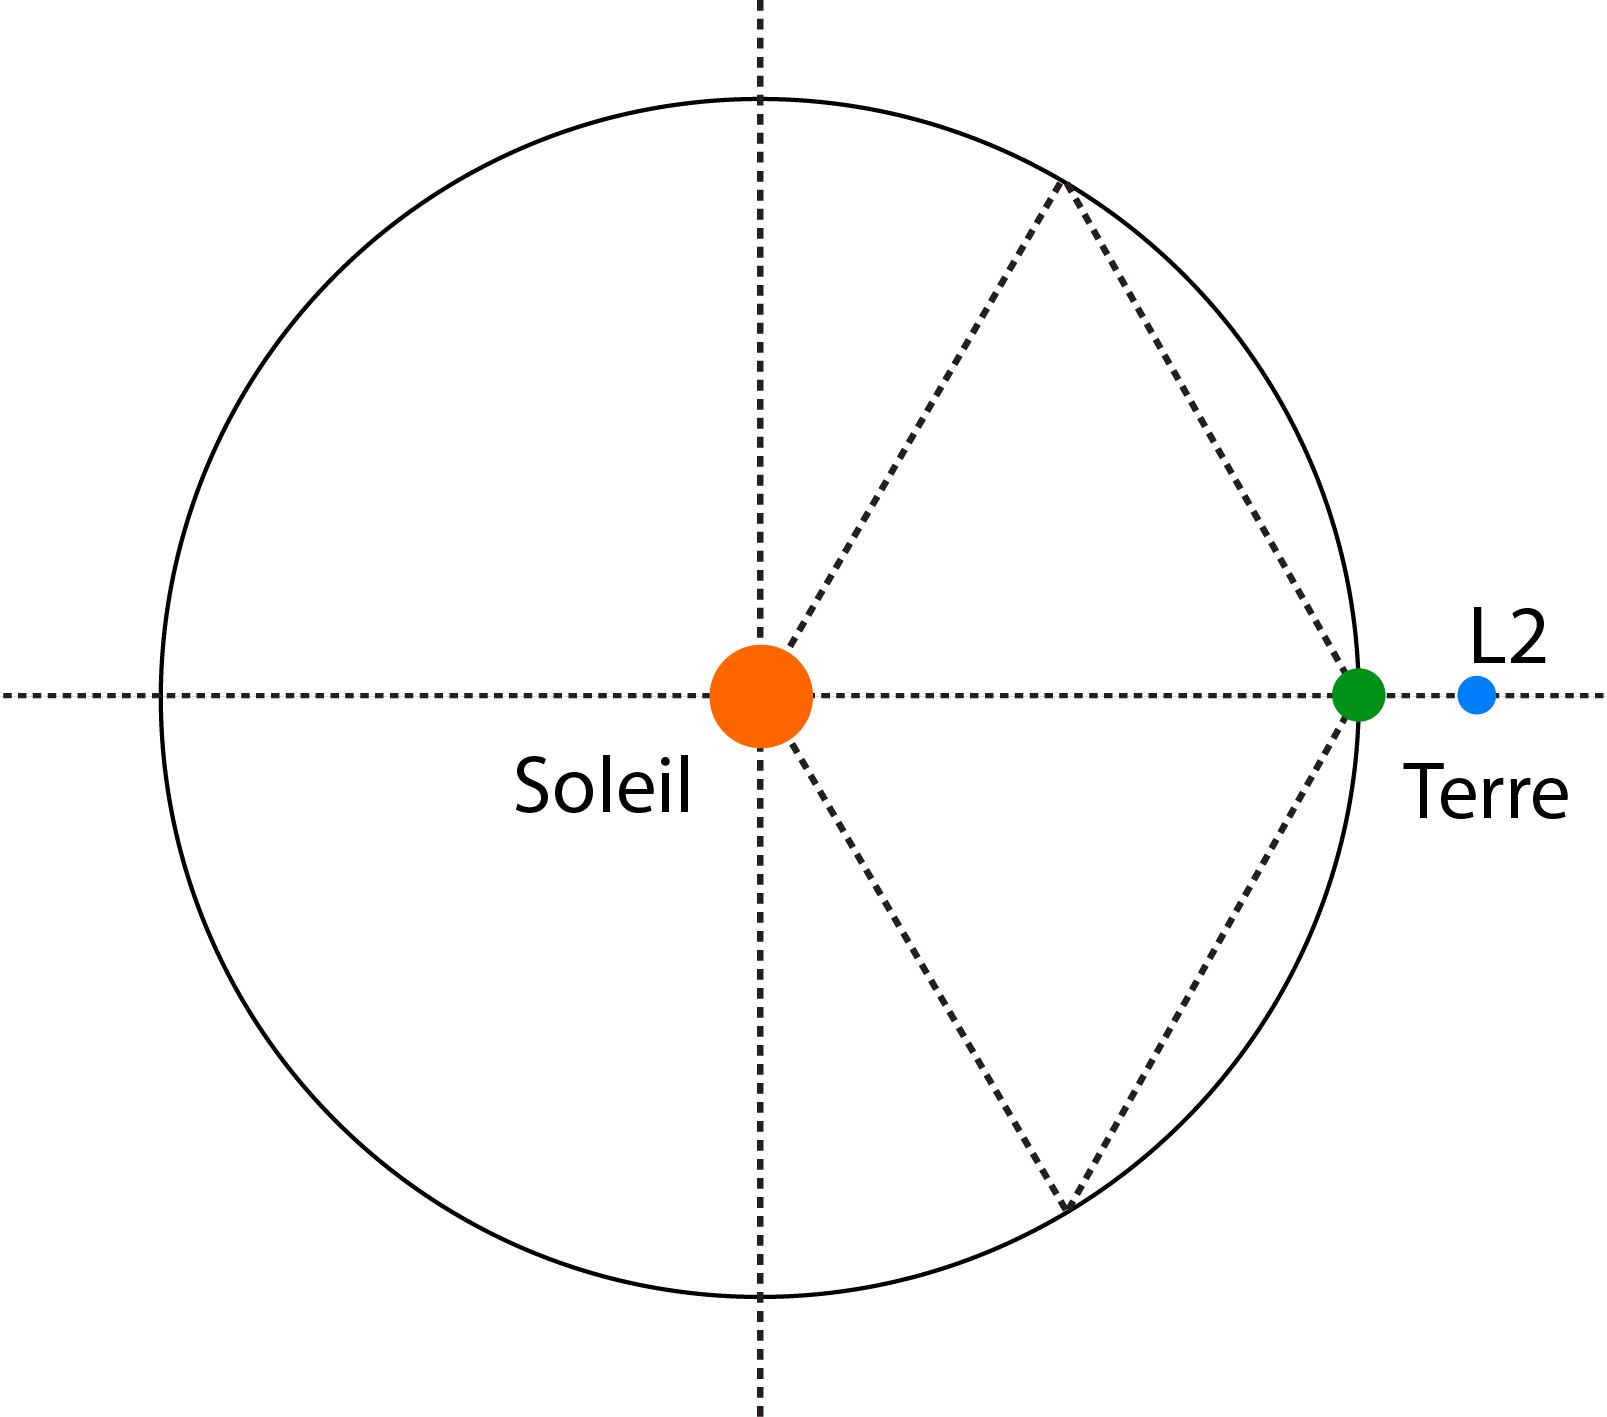
\includegraphics[width=0.6\textwidth]{L2.png}
\caption{Point L2}
\end{figure}
Pour calculer ce point, on supposera que $L1$ et $L2$ sont symétriques par rapport à la Terre. \\
$$\Rightarrow \text{distance soleil} - L2 = R+r$$
On aurait alors les mêmes égalités que pour $L1$, à une exception près : \\
\begin{align*}
\Rightarrow \, &F_{S} = F_{C} + F_{T} \text{ et } vT = 2\pi (R+r)\\
\Rightarrow \, &\boxed{\frac{GM_0}{(R+r)^3} - \frac{GM}{r^2 (R+r)} = \frac{4\pi ^2}{T^2}} \tag{1}
\end{align*}
D'après le calcul du point $L1$ : \\
\begin{equation*}
\Rightarrow \boxed{\frac{GM_{0}M}{R^2} = \frac{Mv^2}{R} = \frac{M4\pi ^2R^2}{RT^2}} \tag{2}
\end{equation*}
On a alors : \\
$$ \frac{GM_0}{(R+r)^3} - \frac{GM}{r^2(R+r)} = \frac{GM_0}{R^3}$$
\[ \text{On pose} : 
\begin{cases}
y = \frac{M}{M_0}  & \quad \text{ très petite valeur}\\
z = \frac{r}{R}  & \quad \text{ petite valeur}\\
\end{cases}
\] 
D'où : 

$$\frac{G}{(R+r)^3} - \frac{G}{r^2(R+r)} *y = \frac{G}{R^3}$$
$$\Rightarrow \text{(Développement limité à l'ordre 1 de }\frac{1}{(1+z)^3} \text{ et } (1+z) \rightarrow 1) $$
$$-3z^3 = y \Rightarrow \boxed{3z^3 = -y}$$
D'où : 
\begin{align*}
&\boxed{r= - \sqrt[3]{\frac{MR^3}{3M_0}}} \\ \\
\Rightarrow \, &\boxed{r =- \sqrt[3]{\frac{(5,972*10^{24})*(1,5*10^8)^3}{3*(1,989*10^{30})}} = -1,5*10^{6}}
\end{align*}
La distance de $L2$ est négative, car $L1$ et $L2$ sont symétriques par rapport à la Terre.
On a donc en réalité $r = 1,5*10^6 $km. L2 est à une distance de $1,5*10^6$ km de la Terre.
\subsection{L3}
\begin{figure}[H]
\centering
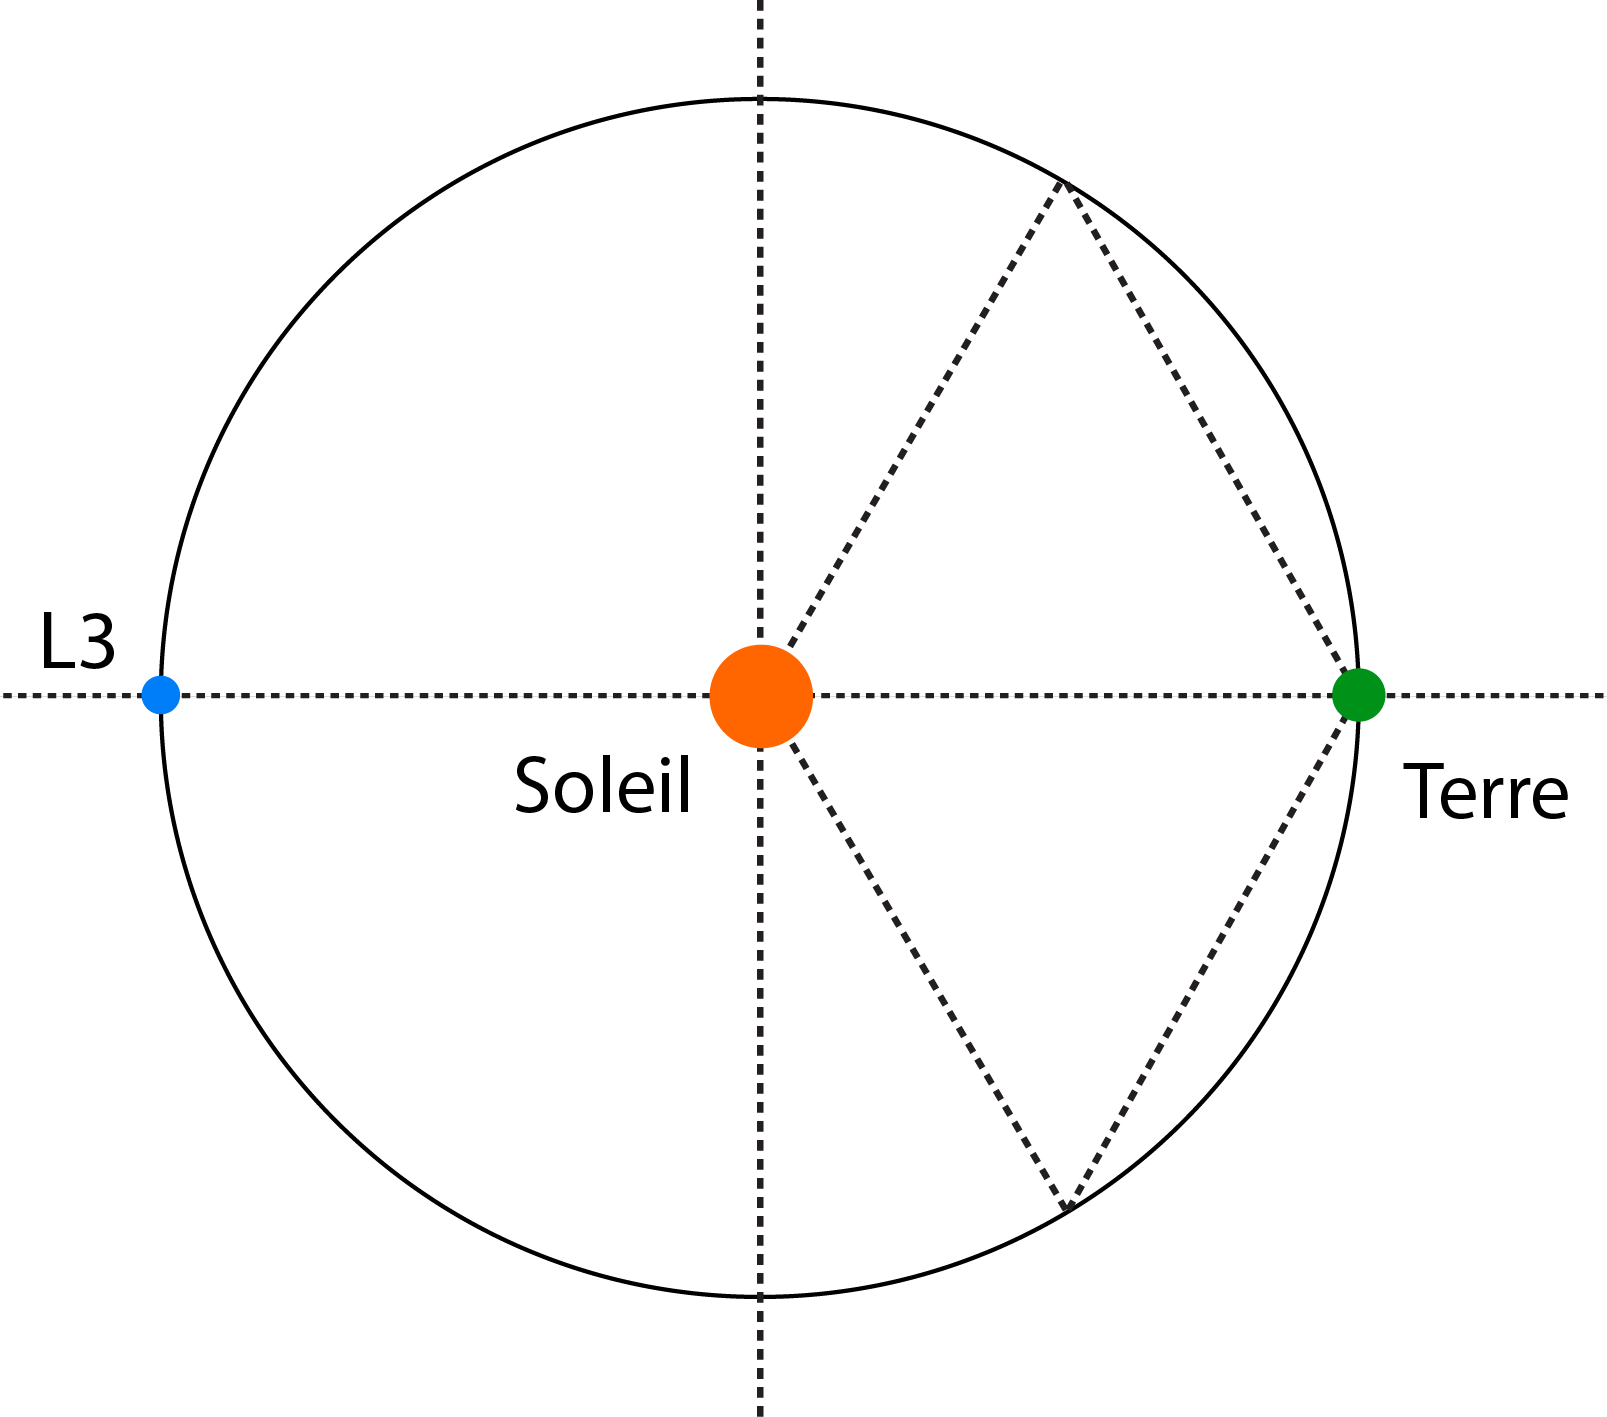
\includegraphics[width=0.6\textwidth]{L3.png}
\caption{Point L3}
\end{figure}
On pose : $a = MM_0$ et $x=L_3M_0-a$ ($x$ est l'écart par rapport à la trajectoire de $M$). \\
$M$ étant très inférieur à $M_0$, le centre de rotation est confondu avec $M_0$. \\
(On néglige l'influence de $M$ sur $M_0$). \\
x est très inférieur à $a$, on pourra donc utiliser l'approximation de Taylor :\\
$$\left(1+ \frac{x}{a}\right)^{-2} = 1 - 2 \frac{x}{a}$$
En $L3$, $m$ subit une force $F_1$ vers $M_0$ et une force $F_2$ vers $M$\\
\begin{align*}
&\bullet \quad F_1 = \frac{GmM_0}{(a+x)^2}\\
&\bullet \quad F_2 = \frac{GmM}{(2a+x)^2}
\end{align*}
\newpage
D'après la 2ème loi de Newton, on a : \\
\begin{align*}
\omega^2 (a + x) &= \frac{(F_1 + F_2 )}{m} \\
&= G\left(\frac{M_0}{(a+x)^2}+\frac{M}{(2a+x)^2}\right)
\end{align*} \\
$m$ devant être fixe par rapport à $M$, il faut que $\omega = \omega_0$ ($\omega_0$ étant la vitesse angulaire de la masse $M$autour de $M_0$).\\ \\
D'après la 2ème loi de Newton, on a également : 
\begin{align*}
&\omega_0^2a = \frac{GM_0}{a^2} \\
\Rightarrow \, &\frac{GM_0(a+x)}{a^3} = G\left(\frac{M_0}{(a+x)^2}\right)
\end{align*} 
En utilisant Taylor, on obtient : 
\begin{align*}
&M_0 \frac{(1 + \frac{x}{a})}{a^2}= M_0\frac{1 - 2 \frac{x}{a}}{a^2} + M\frac{(1 - \frac{x}{a})}{4a^2} \\
\Rightarrow \, &M_0 + M_0 \frac{x}{a} = M_0 - 2M_0 \frac{x}{a} + M(1 - \frac{x}{a})4 \quad \text{et} \quad 3M_0 \frac{x}{a} = \frac{M}{4} \quad \text{(on peut négliger }\frac{x}{a} \text{ devant }1\text{)} \\
\Rightarrow \, &3M_0x = \frac{M}{4}a \\
\Rightarrow \, &3 x = \frac{M}{(4M_0)}a \\
\Rightarrow \, &\boxed{x=\frac{M}{(12M_0)}a}
\end{align*} \\
Pour le système Soleil-Terre, on obtient :
\begin{align*}
x&=2,5*10^{-7} * a\\
&=37,5 \text{ km }
\end{align*}
En réalité, ce point $L3$ n'a pas d'application pratique, il est trop éloigné de M et ne subit pratiquement pas son action. Il est même souvent plus proche des planètes voisines que de $M$ et subit donc davantage leur influence que celle de $M$.
\subsection{L4 et L5}
\begin{figure}[H]
\centering
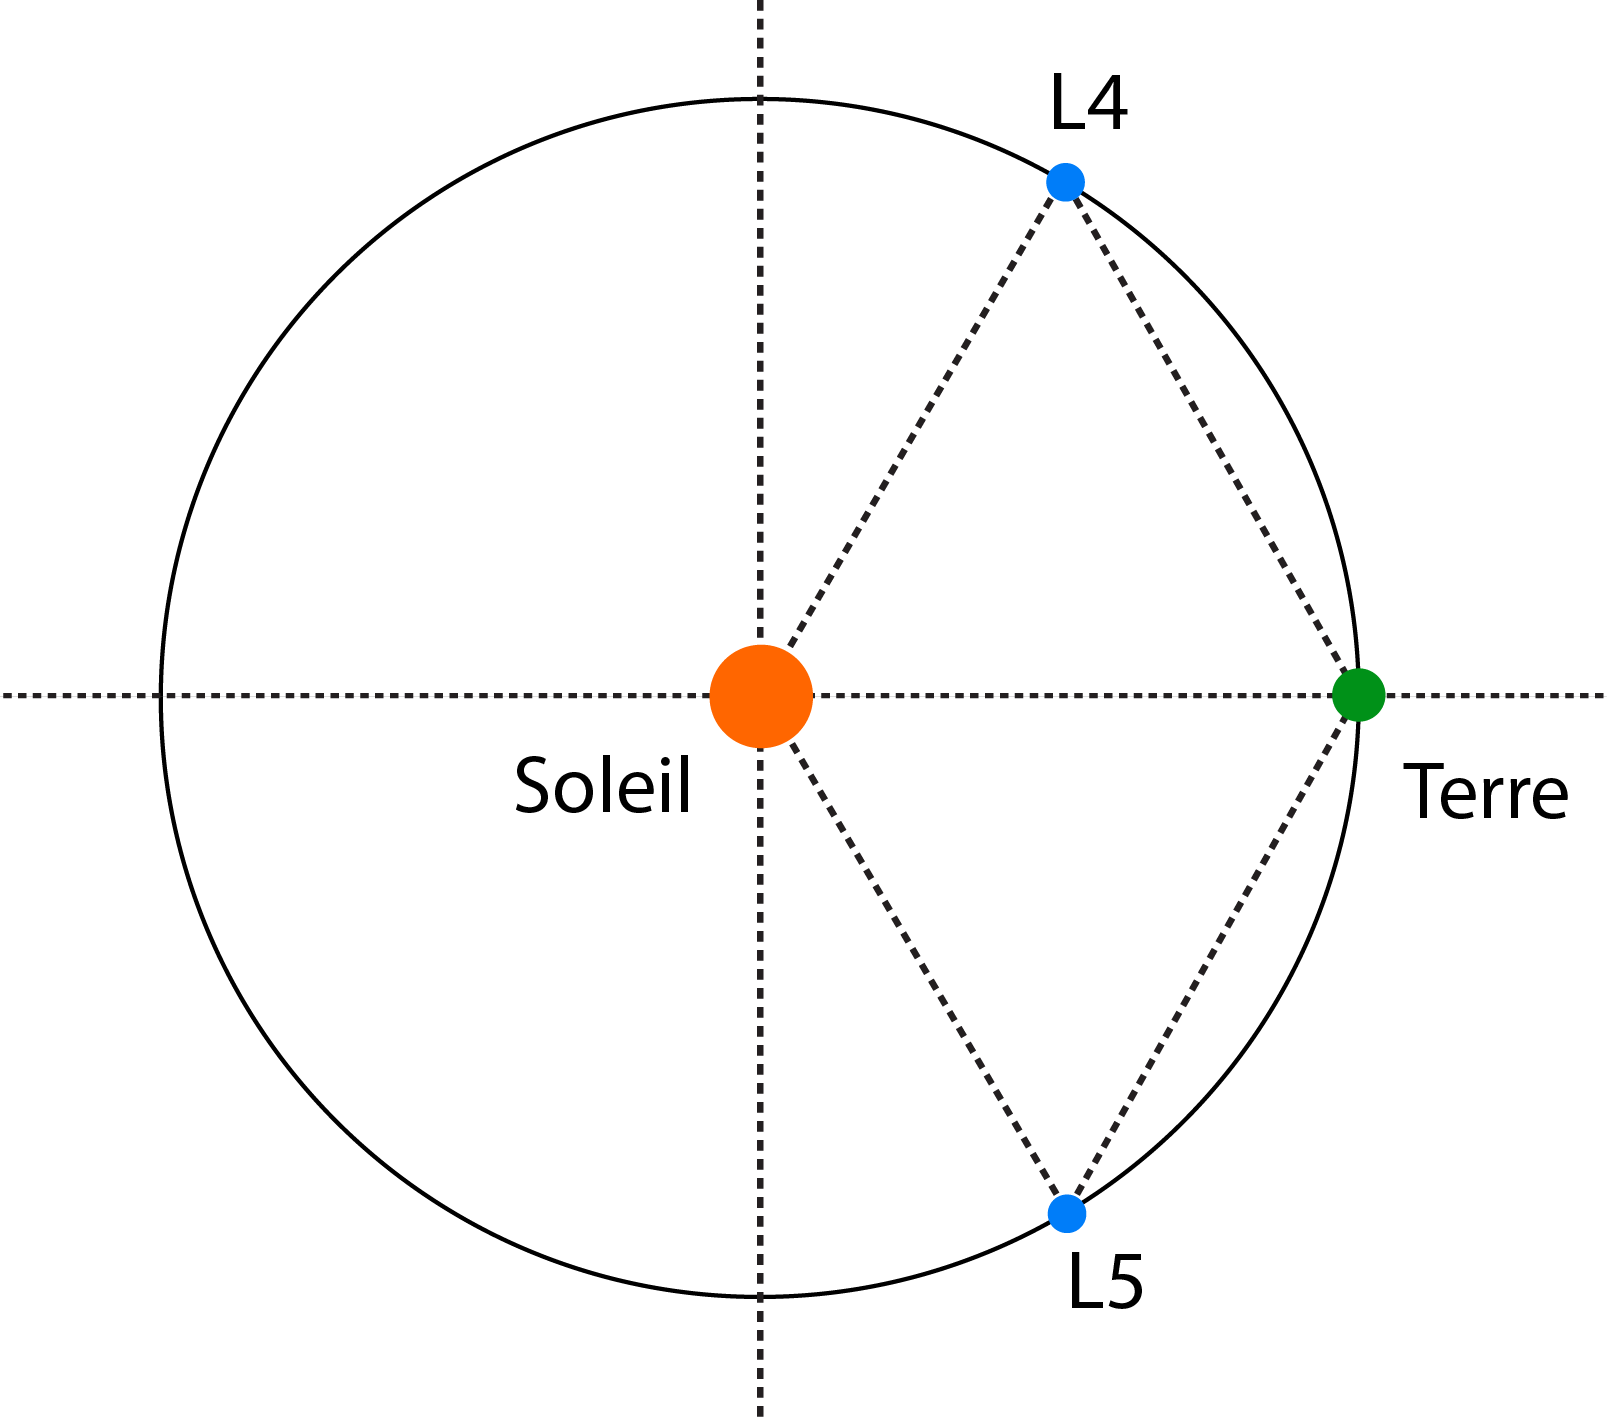
\includegraphics[width=0.6\textwidth]{L4L5.png}
\caption{Points L4 et L5}
\end{figure}
\begin{rappel}[Lois des Sinus]
$$\frac{a}{\sin A} = \frac{b}{\sin B} = \frac{c}{\sin C} $$
\end{rappel}
\begin{figure}[H]
\centering
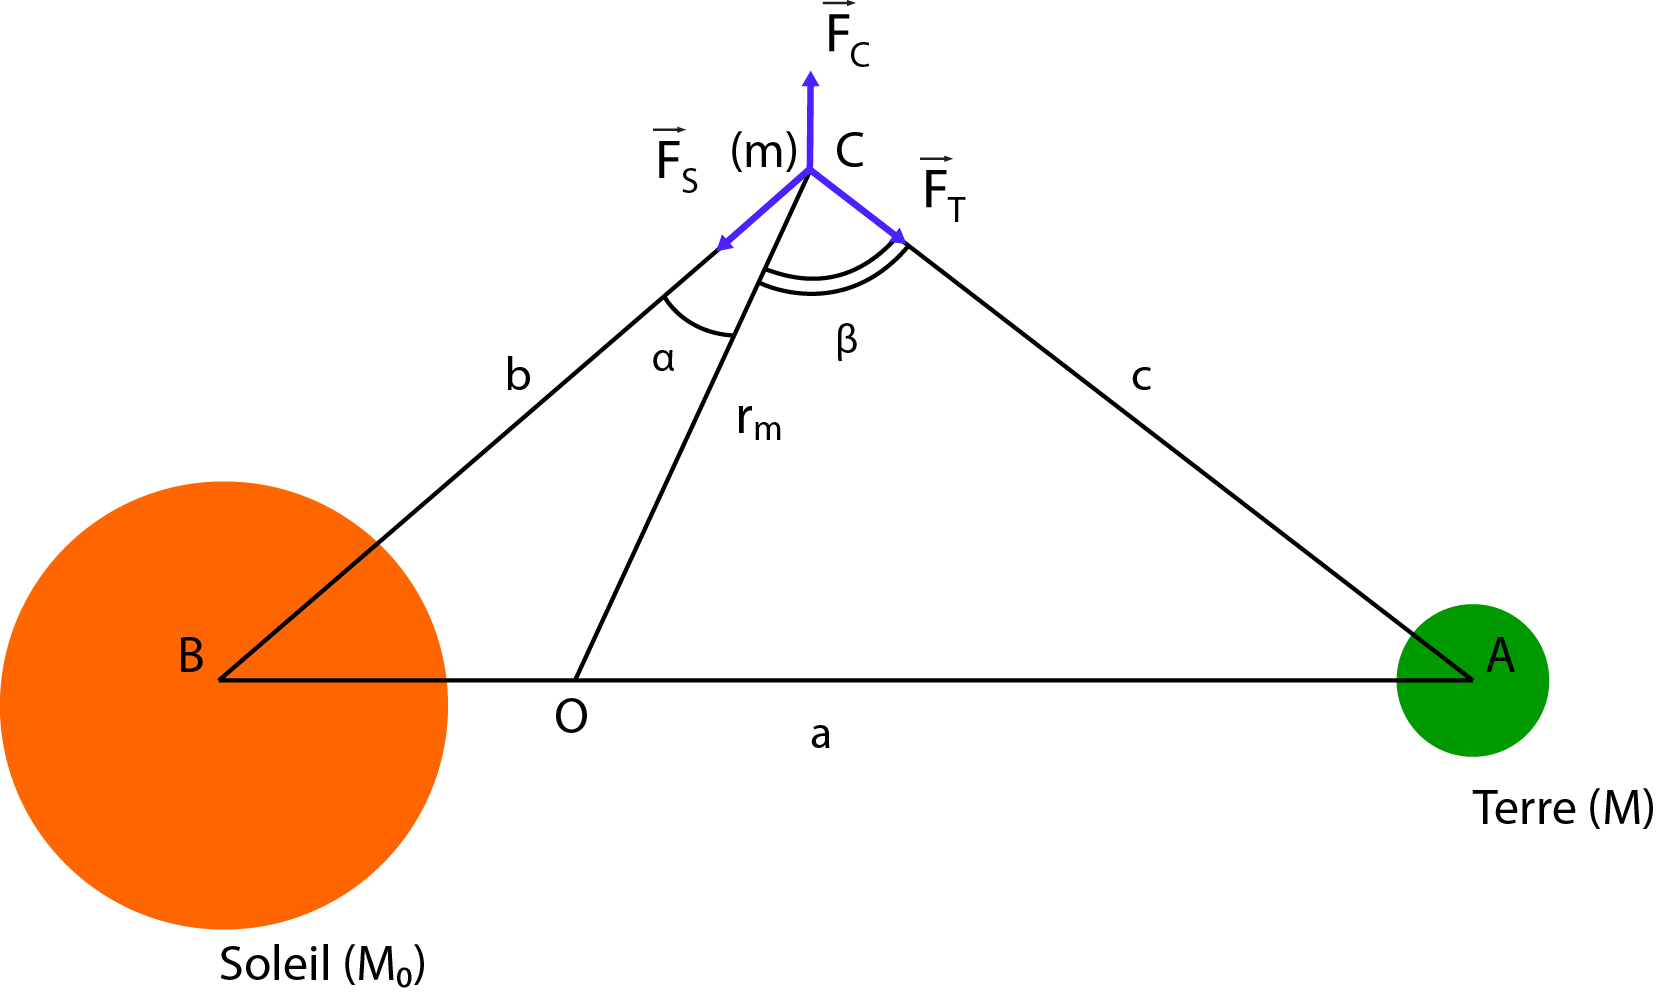
\includegraphics[width=0.9\textwidth]{triangle.png}
\caption{Triangle représentant la Terre, le Soleil et le satellite}
\end{figure}
\[ \text{On pose} : 
\begin{cases}
R = AB \quad \text{avec AB la base du triangle} \\ \\
k = \frac{M}{M_0}\\ \\
OB = \frac{k}{k+1}a \quad OA = \frac{a}{1+k}  \quad \text{ avec a = R}
\end{cases}
\] \\
Nous ajoutons au point $C$ le satellite qui se trouve alors à une distance $b$ du Soleil et à une distance $c$ de la Terre. Le satellite, la Terre et le Soleil forment alors le triangle $ABC$.\\ \\
Nous avons définie $O$ comme le centre d'inertie, ainsi le rayon de rotation m du satellite est différent de celui de la Terre qui est $OA$.
\newpage
Soit $V$ la vitesse de rotation de la Terre et $v$ celle du Satellite : $v = \frac{d}{t} \Rightarrow \boxed{d = vt}$ 
\begin{align*}
\Rightarrow \, &2\pi r_m = vT \text{ et } 2\pi OA = VT \\
\Rightarrow \, &\frac{2\pi}{T} = \frac{v}{r_m} \text{ et } \frac{2\pi}{T} = \frac{V}{a}(1+k)\\
\Rightarrow \, &\boxed{\frac{v}{r_m} = \frac{V}{a}(1+k)} \tag{1}
\end{align*} \\
Par définition, on a la force centrifuge $F_C = m\frac{v^2}{R}$ \\
Donc la force centrifuge sur la Terre est : 
$$F_C = M\frac{V^2}{OA} = M \frac{V^2}{\frac{a}{1+k}} = M\frac{V^2}{a}(1+k)$$ \\
Cette force centrifuge est compensée par la force d'attraction du Soleil sur la Terre $F_S$ : $$ F_S = \frac{GM_0M}{a^2}$$ \\
On a logiquement $F_C = F_S$
$$\Rightarrow \frac{GM_0M}{a^2} = \frac{V^2}{a}(1+k)$$ \\
En multipliant chaque membre par $\frac{a}{M}$ : 
\begin{equation*}
\Rightarrow \boxed{\frac{GM_0}{a} = V^2(1+k)} \tag{2}
\end{equation*} \\ \\
Concernant la force centrifuge sur le satellite : 
$$F_C = m\frac{v^2}{r_m}$$
Elle est équilibrée par la force d'attraction du Soleil et la force d'attraction de la Terre. \\
$$ \vv{F}_{T} = F_T \cos \beta$$
$$ \vv{F}_{S} = F_S \cos \alpha$$\\ 
D'où : 
$$ m\frac{v^2}{r_m} = F_T \cos \beta + F_S \cos \alpha$$
Or, d'après les lois de Gravitation, on a : 
\begin{align*}
&F_T = \frac{GmM}{c^2} \text{\, et \,} F_S = \frac{GmM_0}{b^2}\\
\Rightarrow \, &m\frac{v^2}{r_m} = \frac{GmM}{c^2}\cos \beta + \frac{GmM_0}{b^2} \cos \alpha \\
\Rightarrow \, &\boxed{\frac{v^2}{r_m} = \frac{GM}{c^2} \cos \beta + \frac{GM_0}{b^2} \cos \alpha} \tag{3}
\end{align*}\\
Pour que le satellite soit en équilibre, on doit avoir : 
\begin{align*}
&F_T \sin \beta = F_S \sin \alpha \\
\Rightarrow \, &\frac{GmM}{c^2} \sin \beta = \frac{GmM_0}{b^2} \sin \alpha \\
\Rightarrow \, &\boxed{\frac{M}{c^2} \sin \beta = \frac{M_0}{b^2} \sin \alpha} \tag{4}
\end{align*}\\
On a $(1)$ : 
\begin{align*}
&\frac{v}{r_m} = \frac{V}{a}(1+k) \\
\Rightarrow \, &\frac{v^2}{r_{m}^2} = \frac{V^2}{a^2}(1+k)^2 \\
\Rightarrow \, &\frac{(va)^2}{r_{m}^2} = V^2(1+k)^2 \\
\Rightarrow \, &\frac{(va)^2}{r_m^2(1+k)} = V^2(1+k) \\
\Rightarrow \, &\frac{v^2}{1+k} \frac{a^2}{r_m^2} = V^2(1+k)
\end{align*}
Or $(2)$ : \\
$$\frac{GM_0}{a} = V^2 (1+k)$$ \\
Donc : 
\begin{align*}
 &\boxed{\frac{GM_0}{a} = \frac{v^2}{1+k} \frac{a^2}{r_m^2}} \tag{5} \\ \\
 \Rightarrow \, &\frac{GM_0(1+k)}{a} = \frac{v^2 a^2}{r_m^2} \\
 \Rightarrow \, &\frac{v^2}{r_m^2} = \frac{GM_0(1+k)}{a^3} \Rightarrow \frac{v^2}{r_m} = \frac{GM_0(1+k)r_m}{a^3}
\end{align*} 

Or $(3)$ : 
\begin{align*}
&\frac{v^2}{r_m} = \frac{GM}{c^2} \cos \beta + \frac{GM_0}{b^2} \cos \alpha\\
\Rightarrow \, &\frac{GM_0(1+k)r_m}{a^3} = \frac{GM}{c^2} \cos \beta +\frac{GM_0}{b^2} \cos \alpha \\
\Rightarrow \, &\frac{GM_0}{a^2} \, \frac{r_m}{a} (1+k) = \frac{GM}{c^2} \cos \beta + \frac{GM_0}{b^2} \cos \alpha \\
\Rightarrow \, &\boxed{\frac{1}{a^2} \, \frac{r_m}{a}(1+k) = \frac{1}{c^2}k\cos \beta + \frac{1}{b^2} \cos \alpha} \tag{6}
\end{align*}\\
Supposons que le triangle $ABC$ soit équilatéral, on aurait $a=b=c=u$ avec $u$ d'une certaine longueur et l’on aurait ainsi tous les angles valant $60 \degree$. \\
On aurait alors : 
\begin{align*}
&\frac{1}{a^2} \, \frac{r_m}{a}(1+k) = \frac{k}{a^2} \cos \beta + \frac{1}{b^2} \cos \alpha \\
\Rightarrow \, &\frac{1}{u^2} \, \frac{r_m}{u}(1+k) = \frac{k}{u^2} \cos \beta + \frac{1}{u^2} \cos \alpha \\
\Rightarrow \, &\boxed{\frac{r_m}{u}(1+k) = k \cos \beta + \cos \alpha} \tag{7}
\end{align*}
Or $(4)$ : 
\begin{align*}
&\boxed{\frac{M}{c^2} \sin \beta = \frac{M_0}{b^2} \sin \alpha} \\
\Rightarrow \, &\frac{M}{u^2} \sin \beta = \frac{M_0}{u^2} \sin \alpha \\
\Rightarrow \, &\boxed{M \sin \beta = M_0 \sin \alpha} \tag{8}
\end{align*}\\
On pourra ainsi noter : $ \frac{M}{M_0} = \frac{\sin \alpha}{\sin \beta} \Rightarrow \boxed{k = \frac{\sin \alpha}{\sin \beta}}$ \\ \\
Cela nous donne alors $(7)$ : 
\begin{align*}
&\frac{r_m}{a}(1+k) = \frac{\sin \alpha}{\sin \beta} \cos \beta + \cos \alpha \\
\Rightarrow \, &\sin \beta \frac{r_m}{a}(1+k) = \sin \alpha \cos \beta + \cos \alpha \sin \beta
\end{align*} \\
Rappelons la formule de trigonométrie : 
\begin{align*}
\sin(a+b) &= \sin a\cos b + \cos a\sin b \\
\Rightarrow \sin(\alpha + \beta) &= \sin\alpha\cos\beta + \cos\alpha\sin\beta
\end{align*} \\
D'où : 
\begin{align*}
  \sin\beta \frac{r_m}{a}(1+k) &= \sin(\alpha+\beta) \\
    &= \sin C = \sin A \quad \text{car ABC est équilatéral par hypothèse}
\end{align*}

\begin{align*}
  &\Rightarrow \frac{\sin \beta}{a}(1+k) = \frac{\sin A}{r_m} \\
  &\Rightarrow \frac{\sin \beta}{a}(1+\frac{M}{M_0}) = \frac{\sin A}{r_m} \\
  &\Rightarrow \frac{\sin \beta (M_0+M)}{aM_0} = \frac{\sin A}{r_m} \\
  &\Rightarrow \boxed{\frac{\sin\beta}{\frac{aM_0}{M_0+M}} = \frac{\sin A}{r_m}} \tag{9}
\end{align*} \\
En ayant supposé que le triangle $ABC$ était équilatéral, on a obtenu $(9)$ qui représente la loi des sinus dans le triangle $COA$. Cela implique, que la condition nécessaire pour que toutes nos équations soient vraies, que le triangle $ABC$ soit équilatéral. Par conséquent, le point $L4$ se trouve au point C, sommet du triangle $ABC$ équilatéral de base $ AB = R$. Le triangle étant équilatéral, le point $L4$ se trouve à une unité astronomique et à un angle de $60\degree$ par rapport à l'axe Terre-Soleil. \par Nous savons que les points $L4$ et $L5$ sont les points de Lagrange stables. Or, nous venons de démontrer que, pour qu'un satellite soit stable par rapport à la Terre et au Soleil, il doit être au sommet du triangle équilatéral ayant pour base le segment Terre-Soleil. Par conséquent, soit les points $L4$ et $L5$ sont confondus, soit ils sont symétriques par rapport au segment Terre-Soleil. 
On en conclut alors que le point $L5$ est également à un angle de $60\degree$ par rapport à l'axe Terre-Soleil. $L4$ et $L5$ sont alors symétriques par rapport au segment Terre-Soleil.
\section{Exemples d'applications}
Les points $L1$, $L2$ et $L3$ sont naturellement instables, ce qui signifie que si l'on place un objet à côté de l'un de ces points, il va commencer à s'éloigner de ce point à la moindre perturbation. C'est pour cela que lorsqu'un engin spatial est placé sur l'un de ces points, il doit être stabilisé, on peut par exemple le munir de panneaux solaires qui, en cas de perturbation, donneraient à l'objet l'énergie suffisante pour se stabiliser en ces points. 
Chaque point de Lagrange a une application différente : \\
\begin{itemize}
\item Le point $L1$, est idéal pour observer le Soleil car il tourne continuellement autour de celui-ci. De plus, son champ gravitationnel est relativement faible impliquant une importante économie de carburant en ce point. C'est pourquoi la sonde SOHO y a été installée pour observer le Soleil; \\
\item Le point $L2$ tourne avec la Terre, par conséquent, depuis ce point, le Soleil est constamment caché par la Terre. Ainsi, ce point est idéal pour placer un satellite ayant une direction de visée opposée à la Terre et au Soleil. C'est pour cela que pour la mission Planck le satellite sera placé en ce point afin d'observer l'univers; \\
\item Le point $L3$, quant à lui, est bien trop éloigné de la Terre et nous est invisible car il est derrière le Soleil. Ainsi, il n'y a pas d'application sur ce point; \\
\item Les points $L4$ et $L5$, quant à eux, sont stables. Contrairement à ce que l'on pourrait penser, cette stabilité est plutôt gênante car autour de ces points gravitent de nombreux parasites comme des poussières ou de petits corps célestes qui se retrouveraient piégés en ces points. Par conséquent, on ne peut pas placer d'engins spatiaux dans ces zones car ils ne résisteraient pas aux chocs. 
En réalité, en $L4$ et $L5$ gravitent des astéroïdes que l'on nomme astéroïde troyens (astéroïdes situés sur les points $L4$ et $L5$ du couple Soleil-Terre).
\end{itemize}
\section{Bonus}
\subsection{Énergie Potentielle}
\begin{nota}
Si la somme des forces peut s'annuler, c'est qu'il existe un extremum de l'énergie potentielle.
\end{nota}
On se place comme précédemment dans un repère tournant $(M,M_0)$ :
\begin{align*}
&F_A = \frac{GmM}{c^2} \\
&F_B = \frac{GmM_0}{b^2} \\
&F_C = m\Omega r_m
\end{align*} \\
Ces 3 forces sont conservatrices (ne dépendent pas du temps).\\ On peut les faire dériver d'un potentiel :
\begin{align*}
&\bullet \quad F_A = - \frac{dE_{p_A}}{dG} \Rightarrow \left[E_{p_A} = - \frac{GmM}{c}\right] \quad car \quad F_A = - \frac{GmM}{C} \\
&\bullet \quad F_B = - \frac{GmM_0}{b^2} \Rightarrow \left[E_{p_B} = - \frac{GmM_0}{b}\right] \\
&\bullet \quad F_C = m\Omega^2 r_m = - \frac{dE_{p_m}}{dr_m} \Rightarrow \left[E_{p_m} = -m\Omega^2 \frac{r_m}{2} \right] \\
\end{align*} \\
Donc : 
\begin{align*}
&E_{p_{Totale}} = E_p = E_{p_A} + E_{p_B} +E_{p_m} \\
\Rightarrow \, &E_p = - \left[\frac{GmM}{c} + \frac{GmM_0}{b} + \frac{m\Omega^2 r_m^2}{2}\right] \quad \text{où} \quad \Omega^2 = \frac{G(M+M_0)}{a^3}
\end{align*}
Aussi : 
\begin{align*}
r_A &= \left[(OA-x)^2 +y^2+z^2\right]^{\sfrac{1}{2}} \\
&= \left[\left(\frac{a}{1+k}-x\right)^2+y^2+z^2\right]^{\sfrac{1}{2}}
\end{align*}
(Dans le cas où l'on introduit $c$ comme celui dédié aux coordonnées sphériques) \\
\begin{req}
L'introduction du paramètre est facultative, car on sait d'après le mouvement keplérien que la trajectoire est située dans le même plan. ($z=e$).
\end{req}
\begin{align*}
b &= \left[(OB+x)^2 +y^2+z^2\right]^{\sfrac{1}{2}} \\
&= \left[\left(\frac{ka}{1+k}+x\right)^2+y^2+z^2\right]^{\sfrac{1}{2}}
\end{align*}
$$r_m = (x^2+y^2)^{\sfrac{1}{2}}$$ \\
D'autre part : 
$$ E_{p(x,y)} = - m\Omega^2a^3\left[\left(\frac{k}{1+k}\right) \times \frac{1}{A} + \left(\frac{1}{1+k}\right) \times \frac{1}{B} + \frac{r_m^2}{2a^3}\right]$$
\newpage
\section*{Liens}
https://fr.wikipedia.org/wiki/Force\_centrifuge \\
https://fr.wikipedia.org/wiki/Force\_centripete \\
https://fr.wikipedia.org/wiki/Lois\_du\_mouvement\_de\_Newton \\
https://fr.wikipedia.org/wiki/Point\_de\_Lagrange \\
http://www-spof.gsfc.nasa.gov/stargaze/Slagrang.htm \\
http://hatteras.free.fr/lagrange/lagr01.htm \\
http://www.futura-sciences.com/magazines/espace/infos/dico/d/univers-point-lagrange-4540/ \\
http://gilbert.gastebois.pagesperso-orange.fr/java/poincare/lagrange/lagrange\_theorie.pdf 
\end{document}
